
\setchapterimage[6cm]{cabecera}
\setchapterpreamble[u]{\margintoc}
%%%%%%%%%%%%%%%%%%%%%%%%%%%%%%%%%%%%%%%%%%%%%%%%%%%%%%%%%%%%%

\chapter{Comunicación entre Procesos Remotos }
\label{ch:Comunicación entre Procesos}
\index{Comunicación entre Procesos}

%%%%%%%%%%%%%%%%%%%%%%%%%%%%%%%%%%%%%%%%%%%%%%%%%%%%%%%%%%%%%%%%%%%%%%%%%%%%%%%%%%%%%%%%%%%%%%%%%%%%%%%%%%%%%%%%%%%%%%%%%%%%%%%%%%%%%%%%%%%%%%%%%%%%%%%%%%%%%%%5


\section{Llamados a Procedimientos Remotos (RPC)}
\label{sec:RPC}
\index{RPC}

Se analizan tres aspectos que son importante para comprender este concepto:
\begin{itemize}
	\item el estilo de programación promovido por RPC - programación con interfaces;
	\item la semántica de la llamada asociada con RPC;
	\item  la cuestión clave de la transparencia y su relación con las llamadas a procedimientos remotos.
\end{itemize}

\subsection*{Programaci\'on con Interfases}
\index{Programaci\'on con interfases}

La interfaz de un módulo especifica los procedimientos y las variables a las que se pueden acceder a trav\'es de  otros módulos. 
En sistemas distribuidos las interfaces son  programas distribuidos donde los módulos se ejecutan en procesos separados.
En el modelo cliente-servidor, en particular, cada servidor proporciona un conjunto de procedimientos que están disponibles para uso de los clientes.
\begin{itemize}
	\item No hay detalle de implementación lenguaje de programación. Hay una evolución del software
	\item No hay acceso a variables mediante ejecución de procesos remotos ni mecanismos pase de parámetros (llamada por valor o referencia)
	\item  Direcciones en procesos locales no son válidas en los procesos remotos
	
	\item  Mecanismo RPC se integra con el lenguaje de programación e incluye la notación  para la definición de interfaces con mensajes input/output
	\item Escrita en variedades de lenguajes, C++, Java, Python
	\item Lenguajes de definición de interfaces (IDL) están diseñados para permitir que los procedimientos implementados en distintos lenguajes puedan ser invocados por otros
	
\end{itemize}
%%\subsubsection{Ejemplo: Corba IDL }

%%\index{CORBA}

%%La figura \ref{fig:corba} muestra un ejemplo del lenguaje de definici\'on de interfases \texttt{CORBA}.  La interfase llamada \textit{PersonList} especifica los m\'etodos disponibles para la invocaci\'on remota en el objeto remoto que implementa esa interfase. 
%%El m\'etodo \textit{addPerson} especifica sus argumentos como argumentos de  entrada y el m\'etodo \textit{getPerson} busca una instancia de \textit{Person} por el nombre establecido en su segundo argumento de salida. 


%%\begin{marginfigure}%
%%	\includegraphics {4/Corba.png}
%%	\caption{Ejemplo CORBA. Tomado de \CO}
%%	\label{fig:corba}
%%\end{marginfigure}



\subsection*{Semántica de llamadas de RPC}
\index{sem\'antica de llamadas}

La operaci\'on \textit{doOperation} se puede implementar de diferentes maneras para proporcionar diferentes garantías de entrega en el mensaje (figura \ref{fig:semLLa}). Las principales opciones son:
\begin{itemize}
	\item Reintentar mensaje de solicitud: controlar si se retransmite el mensaje de solicitud hasta se recibe una respuesta o supone que el servidor ha fallado. 
	\item Filtrado duplicado: controlar cuándo se usan las retransmisiones y si se debe filtrar solicitudes duplicadas en el servidor. 
	\item Retransmisión de resultados: controlar si se debe mantener un historial de mensajes de resultados para permitir que los resultados perdidos se retransmitan sin volver a ejecutar las operaciones en el servidor.
\end{itemize}


\begin{marginfigure}%
	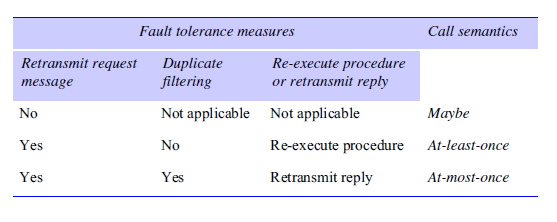
\includegraphics {4/SemanticaLlamadas.png}
	\caption{Semantica de Llamadas de RPC. Tomado de \CO}
	\label{fig:semLLa}
\end{marginfigure}


Con una semántica de Puede ser, el invocador de la llamada recibe un resultado, en cuyo caso el invocador de la llamada  sabe que el procedimiento se ejecutó al menos una vez, o una excepción que le informa que no se recibió ningún resultado. 
Al menos una vez, la semántica puede ser logrado mediante la retransmisión de mensajes de solicitud, que enmascara las fallas de omisión del mensaje de solicitud o resultado. 
La semántica puede sufrir lo siguiente tipos de falla:
\begin{itemize}
	\item fallas de bloqueo cuando falla el servidor que contiene el procedimiento remoto;
	\item fallas arbitrarias: en los casos en que el mensaje de solicitud se retransmite,  el servidor puede recibirlo y ejecutar el procedimiento más de una vez, posiblemente causando valores incorrectos para ser almacenados o devueltos.
\end{itemize}

Con una semántica como máximo, la persona que llama recibe un resultado, en cuyo caso la persona que llama sabe que el procedimiento se ejecutó exactamente una vez, o una excepción que le informa que no se recibió ningún resultado, entonces el procedimiento ha sido ejecutados ya sea una vez o no lo ha sido.




\subsection*{Transparencia}
\index{transparencia}
La elección de si el RPC debe ser transparente también está disponible para los diseñadores de IDL. Por ejemplo, en algunos IDL, una invocación remota puede generar una excepción cuando el cliente no puede comunicarse con un procedimiento remoto. Esto requiere que el programa cliente maneje tales excepciones, permitiéndole lidiar con tales fallas. Un IDL también puede proporcionar una facilidad para especificar la semántica de llamada de un procedimiento. Esto puede ayudar al diseñador del servicio; por ejemplo, si se elige la semántica de llamada al menos una vez para evitar los gastos generales de una vez como máximo, las operaciones deben diseñarse para que sean idempotentes.


\subsection*{Implementaci\'on de RPC}
\index{implementaci\'on de RPC}
El la figura \ref{fig:rpc} se muestra un esquema de los componentes de la arquitectura de RPC. 

El cliente que accede a un servicio incluye un procedimiento \textit{stub} para cada procedimiento definido en la interfaz de servicio. El procedimiento \textit{stub} se comporta como un procedimiento local para el cliente, pero en lugar de ejecutar la llamada, ordena (empaqueta) el identificador del procedimiento y los argumentos en un mensaje de solicitud, que envía a través de su módulo de comunicación al servidor. 


Cuando llega el mensaje de respuesta, desarma (desempaqueta) los resultados. El proceso del servidor contiene un despachador junto con un procedimiento de código auxiliar del servidor y un procedimiento de servicio para cada procedimiento en la interfaz de servicio. El despachador selecciona uno de los procedimientos \textit{stub}  del servidor, según el identificador de procedimiento en el mensaje de solicitud. 

El procedimiento de \textit{stub} del servidor luego  desarma (desempaqueta)  los argumentos en el mensaje de solicitud, llama al procedimiento del servicio correspondiente  y calcula los valores de retorno para el mensaje de respuesta. 

Los procedimientos de servicio implementan los procedimientos en la interfaz de servicio. Los procedimientos de \textit{stub} de cliente y servidor y el despachador puede ser generado automáticamente por un compilador de interfaz a partir de la definición de interfaz del servicio.
RPC generalmente se implementa sobre un protocolo de solicitud-respuesta como los discutidos. 

El contenido de los mensajes de solicitud y respuesta es el mismo que se ilustra para los protocolos de solicitud-respuesta. RPC puede implementarse para tener una de las opciones de semántica de invocación discutidas, generalmente se elige al menos una vez o como máximo una vez. Para lograr esto, el módulo de comunicación implementará las opciones de diseño deseadas en términos de retransmisión de solicitudes, tratamiento de duplicados y retransmisión de resultados.

%%%%%%


\begin{figure}%
	\includegraphics {4/RPC.png}
	\caption{RPC. Tomado de \CO}
	\label{fig:rpc}
\end{figure}
%%%%%%%%%%%%%%%%%%%%%%%%%%%%%%%%%%%%%%%%%%%%%%%%%%%%%%%%%%%%%%%%%%%%%%%%%%%%%%%%%%%%%%%%%%%%%%%%%%%%%%%%%%%%%%%%%%%%%%%%%%%%%%%%%%%%%%%%%%%%%%%%%%%%%%%%%%%


\section{Invocaci\'on a M\'etodos Remotos (RMI)}

Los puntos en común entre RMI y RPC son los siguientes:
\begin{itemize}
	\item Ambos admiten programación con interfaces.
	\item  Están construidos sobre protocolos de solicitud-respuesta y pueden ofrecer un rango de semántica de llamadas como al menos una vez y como máximo una vez.
	\item Ambos ofrecen un nivel similar de transparencia, es decir, las llamadas locales y remotas emplean la misma sintaxis, pero las interfaces remotas suelen exponer la distribución de la llamada subyacente, por ejemplo, admitiendo excepciones remotas.
	
\end{itemize}

Las siguientes diferencias conducen a una mayor expresividad cuando se trata de programación de aplicaciones y servicios distribuidos complejos:

\begin{itemize}
	
	\item El programador puede utilizar todo el poder expresivo de la programación orientada a objetos para  el desarrollo de software de sistemas distribuidos, incluido el uso de objetos, clases y herencia, y también las Metodologías de diseño y herramientas asociadas.
	
	\item  Partiendo del concepto de identidad de objeto en sistemas orientados a objetos, todos los objetos en un sistema basado en RMI tienen referencias de objeto únicas (ya sean locales o remoto), tales referencias de objeto también se pueden pasar como parámetros, ofreciendo así semántica de paso de parámetros significativamente más rica  en RPC.
\end{itemize}


En la figura \ref{fig:invoRem} se hace referencia a los objetos que pueden recibir invocaciones remotas como objetos remotos. Los objetos \textbf{B} y \textbf{F} son objetos remotos. Todos los objetos pueden recibir  invocaciones locales, aunque solo pueden recibirlas de otros objetos que contienen referencias a ellos.  Por ejemplo, el objeto \textbf{C} debe tener una referencia al objeto \textbf{E} para que pueda invocar uno de sus métodos. 

\begin{marginfigure}%
	\includegraphics {4/InvocacionRemota.png}
	\caption{Invocaci\'on Remota. Tomado de \CO}
	\label{fig:invoRem}
\end{marginfigure}

Los siguientes dos conceptos fundamentales están en el corazón del modelo de objeto distribuido: 
\begin{itemize}
	\item Referencias a objetos remotos: otros objetos pueden invocar los métodos de un objeto remoto si tienen acceso a su referencia de objeto remoto. Por ejemplo, un objeto remoto la referencia para B en la Figura   debe estar disponible para A.
	\index{Referencia a objetos remotos}
	\item  Interfaces remotas: cada objeto remoto tiene una interfaz remota que especifica qué de sus métodos se pueden invocar de forma remota. Por ejemplo, los objetos B y F en la Figura   deben tener interfaces remotas. \index{Interfases remotas}
\end{itemize}


Cuando una acción conduce a la instanciación de un nuevo objeto, ese objeto normalmente debe estar  dentro del proceso donde se solicita la instanciación, por ejemplo, donde se utilizó el constructor. 
Si el objeto recién instanciado tiene una interfaz remota, será un objeto remoto con una referencia de objeto remoto.

Las aplicaciones distribuidas pueden proporcionar objetos remotos con métodos para crear instancias de objetos a los que puede acceder RMI, proporcionando así el efecto de manera efectiva de instanciación remota de objetos. 
Por ejemplo, si el objeto L en la figura contiene un método para crear objetos remotos, entonces las invocaciones remotas de C y K podrían conducir a la instanciación de los objetos M y N, respectivamente. (ver figura \ref{fig:instan})


\begin{marginfigure}%
	\includegraphics {4/Instancia.png}
	\caption{Instaciaci\'on Remota. Tomado de \CO}
	\label{fig:instan}
\end{marginfigure}


\subsection*{Arquitectura RMI}

La arquitectura se muestra en la figura \ref{fig:rmi}

\begin{description}
	\index{Arquitectura de RMI}
	\item[Módulo de Comunicación] Proporcionan semántica de invocación, como ejemplo, al-menos-uno
	Transmite mensaje de solicitud/respuesta entre cliente y servidor
	Solicitud es (tipo de mensaje, IdSolicitud, ref objeto remoto, IdOperacion, Argumentos)
	En el servidor selecciona el despachador para la clase de objeto que se invoca. 
	El despachador ubica la referencia local del objeto en el Módulo de Referencia Remota
	
	
	\begin{figure}%
		\includegraphics {4/RMI.png}
		\caption{Arquitectura RMI. Tomado de \CO}
		\label{fig:rmi}
	\end{figure}
	
	\item[Módulo de Referencia Remota] Responsable de trasladar referencias de objetos locales a remotas y creación de referencias remotas
	Contiene una  tabla de objetos remotos y una tabla para cada proxy local
	Actúa de la manera siguiente:
	\begin{itemize}
		\item 1era vez cuando se pasa un objeto remoto, el módulo de referencia remota crea una referencia al objeto remoto y se añade a la tabla de objetos remotos
		\item Cuando llega referencia a un objeto remoto, el módulo de referencia obtiene referencia al objeto local, la cual es un proxy o un objeto remoto. Si el objeto remoto no está en la tabla se crea el proxy y se añade el módulo de referencia remota
	\end{itemize}
	
	\item[Criado (servant)] Instancia de una clase que proporciona el cuerpo de un objeto remoto. 
	Maneja el requerimiento remoto pasado por el esqueleto              correspondiente. Se crea cuando se instancia el objeto remoto. 
	
	\item[Proxy]
	Proporciona que los métodos de invocación remota sean                 transparente al usuario comportandose como un objeto local.
	Esconde los detalles del empaquetamientos- desempaquetamiento de las referencias a objetos remotos.
	
	\item[Despachador] 
	Un servidor tiene un despachador y un esqueleto.
	Recibe la petición desde el  módulo de comunicación.
	Usa el IdOperacion para seleccionar el método adecuado en el esqueleto
	
	\item[Esqueleto] 
	Implementa el método  en la interface remota. 
	Desempaqueta los argumentos e invoca el método      				correspondiente en el criado.
	Espera que la invocación se complete y empaqueta los resultados
\end{description}


\subsection*{Colector de Basura Distribuida} 
\index{Colector de basura distribuida}
Es un algoritmo distribuido cuya funci\'on es  recolectar la basura distribuida. Establece una cooperación entre el colector local y un módulo añadido que colecciona la basura distribuida

Colector de basura distribuida:
\begin{enumerate}
	\item  Cada proceso servidor mantiene un conjunto de nombres de los procesos que proporcionan referencias a objetos remotos por cada uno de sus objetos remotos. Este conjunto se puede almacenan en una columna adicional de la tabla de objetos remotos.
	\item Cuando un cliente C recibe una referencia remota a un objeto remoto en particular, B,  hace una invocación AddRef (B) al servidor de ese objeto remoto y luego crea un proxy; el servidor agrega un apuntador C a B.
	\item  Cuando  recolector de basura de un cliente C nota que un proxy de un objeto remoto B no está accesible, hace una invocación removeRef (B) al servidor correspondiente y luego borra el proxy; el servidor elimina apuntador C de B.
	\item Cuando apuntador B está vacío, el recolector de basura local del servidor recuperará el espacio ocupado por B a menos que existan apuntadores locales.
\end{enumerate}

\section{Caso de Estudio: Web Socket}